\documentclass[12pt]{article} % Default font size is 12pt, it can be changed here
\usepackage{fontspec}
%Ligatures=TexOff disable the Tex specific ligatures which converst quotes into typographic quotes
\setmainfont{OpenSans}[Ligatures=TeXOff, Path=fonts/,Extension=.ttf, UprightFont=*-Regular, ItalicFont=*-Italic, BoldFont=*-Bold, BoldItalicFont=*-BoldItalic]
\usepackage{microtype}

%\usepackage{tabulary}
\usepackage{tabu} %span tables over multiple pages while still wrapping text inside cells
\usepackage{longtable} %needed by tabu package
\usepackage{geometry}
\geometry{a4paper, total={170mm,257mm}, left=20mm, top=20mm, }

\usepackage{graphicx} % Required for including pictures
\usepackage{tikz}
\usepackage{float} % Allows putting an [H] in \begin{figure} to specify the exact location of the figure
\usepackage{wrapfig} % Allows in-line images such as the example fish picture
\usepackage{lipsum} % Used for inserting dummy 'Lorem ipsum' text into the template
\usepackage{xparse} % Used for defining new commands with arguments

\newcommand{\sectionbreak}{\clearpage}

\graphicspath{{../graphics/}} % Specifies the directory where pictures are stored 

\usepackage{tcolorbox}
\tcbuselibrary{skins}

\usepackage{listings} % Code listings
\usepackage{color}
\definecolor{lightgray}{rgb}{.9,.9,.9}
\definecolor{darkgray}{rgb}{.4,.4,.4}
\definecolor{purple}{rgb}{0.65, 0.12, 0.82}
\definecolor{orange}{rgb}{1, 0.4, 0.0}

\lstdefinelanguage{JavaScript}{
    keywords={typeof, new, true, false, catch, function, return, null, catch, switch, var, if, in, while, do, else, case, break},
    keywordstyle=\color{blue}\bfseries,
    ndkeywords={class, export, boolean, throw, implements, import, this},
    ndkeywordstyle=\color{darkgray}\bfseries,
    identifierstyle=\color{black},
    sensitive=false,
    comment=[l]{//},
    morecomment=[s]{/*}{*/},
    commentstyle=\color{orange}\ttfamily,
    stringstyle=\color{purple}\ttfamily,
    morestring=[b]',
    morestring=[b]"
}

\lstset{
    language=JavaScript,
    backgroundcolor=\color{blue!5},
    extendedchars=true,
    basicstyle=\scriptsize\ttfamily,
    showstringspaces=false,
    showspaces=false,
    tabsize=4,
    breaklines=true,
    showtabs=false,
    captionpos=b,
    frame=leftline,
    rulecolor=\color{blue!20},
    framerule=2pt
}
\setlength{\parindent}{0pt} % removes the default indentation of first lines
\setlength{\tabcolsep}{12pt}

\newenvironment{mono}{\ttfamily}{\par}
\newenvironment{keyword}{\leavevmode\color{magenta}\ttfamily}{}
\newenvironment{keywordpurple}{\leavevmode\color{purple}}{}
\newenvironment{examplecomment}{\leavevmode\color{magenta!60!white}}{}
\newenvironment{code}{\begin{mdframed}[linewidth=4pt, linecolor=blue!40, topline=false, bottomline=false, rightline=false, backgroundcolor=blue!10]
                          \begin{mono}}{\end{mono}
\end{mdframed}}

\newenvironment{properties}
{
    \footnotesize\renewcommand{\arraystretch}{1.30}
    \renewcommand{\tabcolsep}{0pt}
    \begin{longtable}{>{\begin{keyword}}p{3.1cm}<{\end{keyword}}p{13.9cm}}
        \hline
        }
        {
        \hline
    \end{longtable}\vspace{5mm}
}

\newenvironment{parameters}
{
    \footnotesize\renewcommand{\arraystretch}{1.30}
    \renewcommand{\tabcolsep}{0pt}
    \begin{longtable}{>{\begin{keyword}}p{3cm}<{\end{keyword}}>{\begin{em}}p{1.5cm}<{\end{em}}p{12.5cm}}
        \hline
        }
        {
        \hline
    \end{longtable}\scriptsize\vspace{-5mm}*mandatory parameters\vspace{5mm}
}

\NewDocumentEnvironment{variable_properties}{mm} % two mandatory args
{
    \footnotesize\renewcommand{\arraystretch}{1.30}
    \renewcommand{\tabcolsep}{0pt}
    \begin{longtable}{>{\begin{keyword}}p{#1}<{\end{keyword}}p{#2}}
        \hline
        }{
        \hline
    \end{longtable}\vspace{5mm}
}

\newtcolorbox{exampleResultBox}[2][]{
    skin=bicolor,colback=magenta!10!white,
    fonttitle=\bfseries,
    colbacktitle=magenta,
    bottomtitle=2mm,
    toptitle=2mm,
    colbacklower=black!10!white,
    title=#2,#1,
    boxrule=0mm,
    middle=0mm,
    boxsep=0mm,
    left=5mm,
    right=5mm,
    bottom=5mm,
    top=5mm,
    after upper={\hyphenpenalty=10000\raggedright\vskip 5mm\null},
    subtitle style={colback=black,left=5mm,right=5mm,bottom=2mm,top=2mm}
}

\newtcolorbox{exampleBox}[2][]{
    colback=magenta!10!white,
    fonttitle=\bfseries,
    colbacktitle=magenta,
    boxrule=0mm,
    title=#2,#1
}

\newtcolorbox{resultBox}[2][]{
    colback=black!20!white,
    fonttitle=\bfseries,
    colbacktitle=black,
    boxrule=0mm,
    title=#2,#1
}

\newtcolorbox{advancedBox}[2][]{
    colback=purple!10!white,
    fonttitle=\bfseries,
    colbacktitle=purple,
    boxrule=0mm,
    title=#2,#1
}

\newtcbox{\tokenbox}{
    on line,
    colback=magenta,
    coltext=white,
    boxrule=0pt,
    arc=5pt,
    boxsep=1pt,
    left=3pt, right=3pt,
    top=1pt, bottom=1pt,
    tcbox raise base,
    enhanced,
    before=\hspace{2pt}, % space before box
    after=\hspace{2pt}, % space after box
}

\newcommand{\token}[1]{\tokenbox{\MakeUppercase{#1}}}

\setlength{\parskip}{-0.2cm}

\DeclareTextFontCommand{\kw}{\keyword}
\DeclareTextFontCommand{\kwp}{\keywordpurple}

\begin{document}
    \small

%----------------------------------------------------------------------------------------
%	TITLE PAGE
%----------------------------------------------------------------------------------------

    \begin{titlepage}

        \newcommand{\HRule}{\rule{\linewidth}{0.5mm}} % Defines a new command for the horizontal lines, change thickness here

        \center % Center everything on the page

        \begin{tikzpicture}[remember picture,overlay]
            \node[anchor=north west,inner sep=1cm] at (current page.north west){
\includegraphics[width=3cm]{logos/UniLogo}};
        \end{tikzpicture}

        \begin{tikzpicture}[remember picture,overlay]
            \node[anchor=north east,inner sep=1cm] at (current page.north east){
\includegraphics[width=6cm]{logos/LUCET}};
        \end{tikzpicture}\\[6cm]

        {\large OASYS v3.6.0}\\[0.5cm] % Software version this document applies to

        \HRule \\[0.4cm]
        { \huge \bfseries Scripting}\\[0.4cm] % Title of document
        \HRule \\[1.5cm]

        \large
        \textit{Author:} Eric J. FRANCOIS % Your name
        \begin{tikzpicture}[remember picture,overlay]
            \node[anchor=south,inner sep=2cm] at (current page.south){\large \today};
        \end{tikzpicture}

    \end{titlepage}

    \newpage


    \section{description}\label{sec:description}

    Scripting in OASYS is used predominantly to implement conditional branching in an otherwise linear test.
    It can read variables and act according to conditions linked to these variables.\\

    It can also reset variables, for instance when a test is used for learning purposes and you want to loop back before an example item that was answered incorrectly.\\

    Some arithmetic operations are also available, such as calculating sums and averages.\\

    Finally, some internal variables of the test and the platform can be read and acted upon, such as the type of device running the test and more \ldots\\

    Scripts cannot, however, read the score of the test. This limitation is currently in place to avoid the risk of cheating by reading the score in the debugger of the browser and acting upon it.\\
    This may be subject to change in the future, but for now, scripts can only react directly to the value of given answers, not to the score attributed to them.\\


    \section{context}\label{sec:context}

    There are 4 different contexts in which scripts can be used:\\
    \begin{itemize}
        \item \textbf{when navigating to a page} – this is used mainly to check if this page needs to be skipped in case of conditional branching, for instance if the questions only apply to those people who answered in a specific way to a previous question.
        \item \textbf{on input} – this script is executed when the user inputs an answer, for instance to set a variable based on the input.
        \item \textbf{when leaving a page} – on leaving a page, this script is executed, for instance to check if the user is sent back if they answered the example question incorrectly. It can also be used for more complex branching than just skipping the next page.
        \item \textbf{visibility conditions} – this script executes both on navigating to a page and on input, and is used to determine if a given element should be visible or not. This is a lighter way to implement conditional visibility, as it is integrated directly in the content editor and does not require a separate script to be written.
    \end{itemize}


    \section{variables}\label{sec:variables}

    \subsection{variable types}\label{subsec:variable_types}

    There are 3 different types of variables in OASYS:\\
    \begin{itemize}
        \item \textbf{internal variables} – these are variables that are set by the platform, such as the device type, selected options for the test and overrides for the current test taker, etc. They can be read but not set.
        \item \textbf{local variables} – these are answers given by the test taker on the current page, such as the answer to a question or the value of a slider. They can be read and set, but only on the current page.
        \item \textbf{global variables} – these are answers given by the test taker anywhere in the test, such as the answer to a question on a previous page. In order to make them available throughout the test, they need to be exported to a unique variable name, which is then used to read and set the value of the variable. Global variables can be read and set anywhere in the test.
    \end{itemize}

    When reading a variable, local variables start with two dollar signs: \kw{\$\$variable\_name}; while global variables start with a single dollar sign \kw{\$variable\_name}.\\
    Internal variables start with a dollar followed by two underscores \kw{\$\_\_variable\_name}.\\

    \subsection{exporting global variables}\label{subsec:exporting_global_variables}

    In order to export a local variable to a global variable, go to the properties of an interaction, open the \kw{Scripting} section and enter the desired export name into the export field.\\

    \begin{figure}[H]
        \centering
        \fbox{
            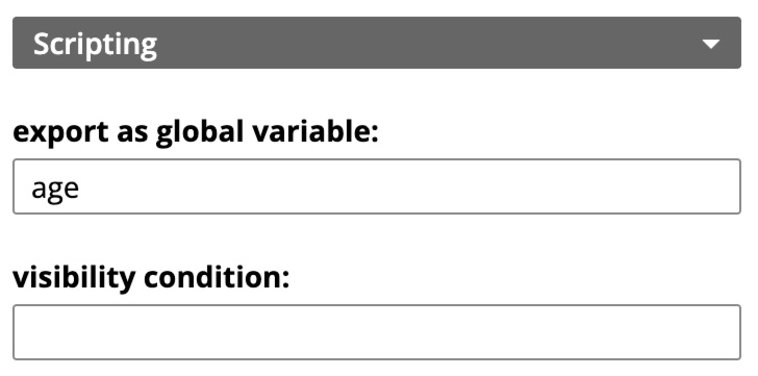
\includegraphics[width=9cm, page=1]{scripting_export_var}
        }
        \caption{Exporting an interaction to a global variable}
        \label{fig:export_global_variable1}
    \end{figure}
    \vspace{0.5cm}

    In the advanced editor, this is done by adding a \kw{EXPORT="variable\_name"} attribute to the code of the field. In case of a radio button group or a checkbox group, it's sufficient to add the attribute only in the first field of the group.\\

    \begin{figure}[H]
        \centering
        \fbox{
            \includegraphics[width=14cm, page=2]{scripting_export_var}
        }
        \caption{Exporting an interaction to a global variable in the advanced editor}
        \label{fig:export_global_variable2}
    \end{figure}
    \vspace{0.5cm}

    The export name must be unique, and it is recommended to use a descriptive name that indicates the purpose of the variable. Since pages are edited outside of the scope of a test, OASYS is not able to check for uniqueness of the variable name. This responsibility lies with the test author.\\

    \textbf{Beware:} Meta fields like choice matrix or inline fields, where a single interaction creates multiple local variables, cannot be exported to global variables at the moment.\\


    \section{creating a script}\label{sec:creating_a_script}

    \subsection{creating a script in the test manager}\label{subsec:creating_a_script_in_the_test_manager}

    In the test manager create a structure and then click on the script button of the page you want to create a script for.\\

    \begin{figure}[H]
        \centering
        \fbox{
            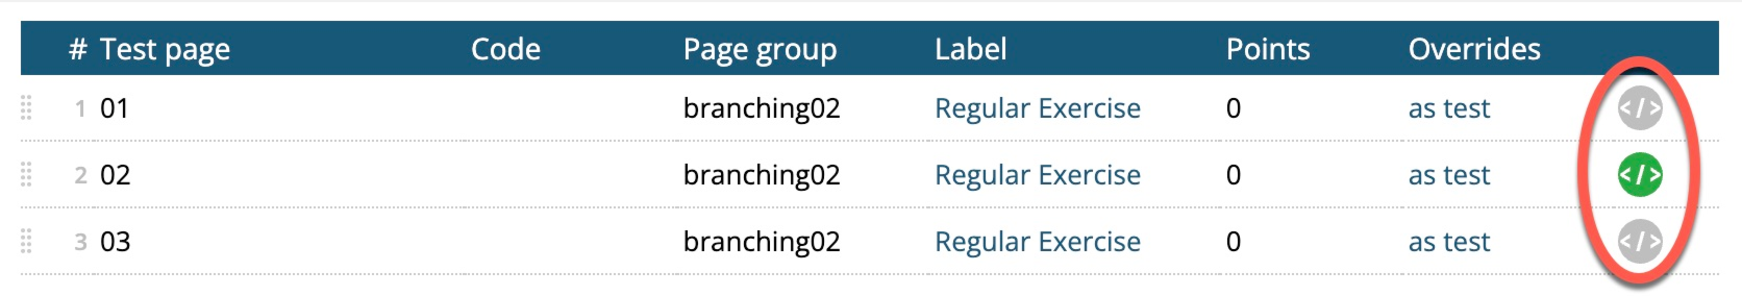
\includegraphics[width=15cm]{scripting_testEditor}
        }
        \caption{Creating a script for a page}
        \label{fig:create_script}
    \end{figure}
    \vspace{0.5cm}

    Then you can choose between three tabs \kw{Pre}, \kw{Post}, \kw{on Activity} to define scripts for different points in time. The "Pre" script will be evaluated when you are navigating to this page, the "Post" one will be run when navigating away from the page and "on Activity" will be run when an answer is given or edited.

    \begin{figure}[H]
        \centering
        \fbox{
            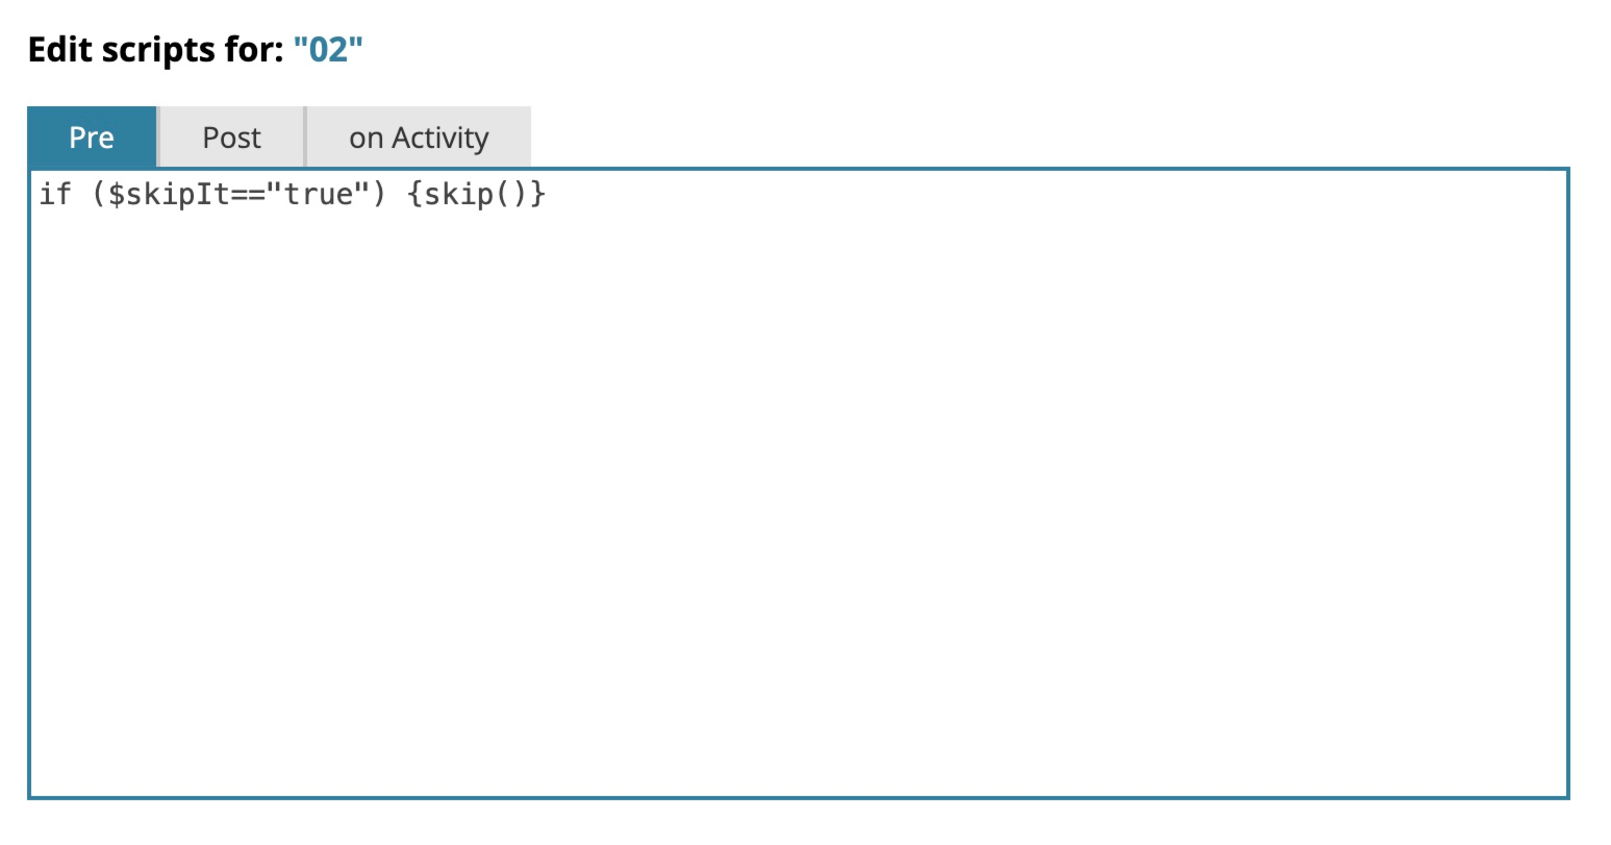
\includegraphics[width=15cm]{scripting_contexts}
        }
        \caption{Choosing the context of a script}
        \label{fig:script_tabs}
    \end{figure}
    \vspace{0.5cm}

    \subsection{creating a visibility condition in an interaction}\label{subsec:creating_a_visibility_condition_in_an_interaction}

    In the interaction editor, you do not have to create a complete script, but only a condition that will be evaluated to determine if the block is visible or not.\\

    \begin{figure}[H]
        \centering
        \fbox{
            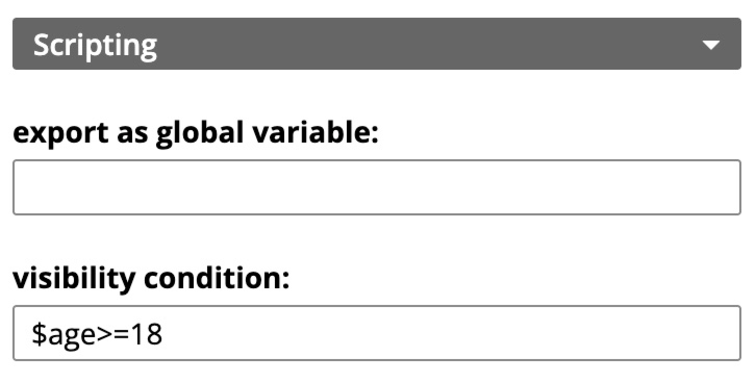
\includegraphics[width=9cm]{scripting_visibility}
        }
        \caption{Creating a visibility condition in an interaction}
        \label{fig:visibility_condition}
    \end{figure}


    \section{syntax of a script}\label{sec:syntax_of_a_script}

    \subsection{structure of a command}\label{subsec:structure_of_a_command}
    Currently, 3 base commands are available in OASYS scripts:
    \begin{itemize}
        \item \textbf{IF/ELSE} – this command is used to check a condition and execute a block of code if the condition is true and execute another block of code if the condition is false.
        \item \textbf{IF} – this command is used to check a condition and execute a block of code if the condition is true. If the condition is false, the script will continue to the next command without executing any code.
        \item \textbf{EXECUTE} – this command is used to execute a block of code without conditions.
    \end{itemize}
    \vspace{0.5cm}

    The structures of those commands are as follows:\\

    {\large
        \begin{center}
            if (\token{condition}) \{\token{action}\} else \{\token{action}\} \\[0.2cm]
            if (\token{condition}) \{\token{action}\} \\[0.2cm]
            execute \{\token{action}\} \\[0.2cm]
        \end{center}
    }

    \subsection{syntax of a condition}\label{subsec:syntax_of_a_condition}

    The main syntax of a condition is as follows:\\
    {\large
        \begin{center}
            \token{term1} \token{operator} \token{term2}\\[0.2cm]
        \end{center}
    }

    The terms can be either a global or local variable as shown previously, strings, numbers, or the result of the \kw{count} command.

    \begin{variable_properties}{3.5cm}{13.5cm}
        \hline
        \$\$variable & local variable, e.g.\ the answer to a question on the current page, where the variable name corresponds to the field id; they always start with two dollar signs\\
        \$variable & global variable, e.g.\ the answer to a question on a previous page, where the variable name corresponds to the export name of the field; they always start with a single dollar sign\\
        \$\_\_variable & internal variable, e.g.\ the device type, where the variable name corresponds to the name of the internal variable; they always start with a dollar sign followed by two underscores\\
        "string" or 'string' & a string, written either with double or single quotes, e.g.\ "hello world" or 'hello world' \textit{(please make sure to use straight quotes, not curly ones)}\\
        42 & a number, which can be either an integer or a float, e.g.\ 42 or 3.14 (please make sure to use a dot as decimal symbol, not a comma)\\
        count(\$variable) & the number of answers in an array-type field, or 1/0 depending on whether any other field type has been answered; the variable can be global or local\\
        \hline
    \end{variable_properties}
    \vspace{0.1cm}

    Multiple conditions can be combined using the logical operators \kw{\&\&} and \kw{||} for "and" and "or" respectively.\\

    \begin{exampleBox}{Example}
        Checking if age is between 13 and 17:\\[0.2cm]
        \kw{if (\$\$age >= 13 \&\& \$\$age <= 17) \{\ldots\}}\\[0.5cm]
        Checking if at least two answers are selected in a checkbox group:\\[0.2cm]
        \kw{if (count(\$\$checkboxes) >= 2) \{\ldots\}}\\
    \end{exampleBox}

    \subsection{syntax of an operator}\label{subsec:syntax_of_an_operator}

    The operators are used to compare the terms in a condition. The following operators are available:\\
    \begin{variable_properties}{2.5cm}{14.5cm}
        \hline
        == & equal to (for numbers or strings)\\
        != & not equal to (for numbers or strings)\\
        < & less than (only for numbers)\\
        <= & less than or equal to (only for numbers)\\
        > & greater than (only for numbers)\\
        >= & greater than or equal to (only for numbers)\\
        contains & true if a group contains a specific value (only for array-type answers like checkboxes)\\
        !contains & true if a group does not contain a specific value (only for array-type answers like checkboxes)\\
        \hline
    \end{variable_properties}

    \subsection{defined actions}\label{subsec:defined_actions}

    A set number of actions are available in OASYS scripts. They can be used in the \kw{execute} command or in the \kw{if} and \kw{else} blocks.\\

    Some commands need parameters, which are given within parentheses after the command name, separated by commas. Beware that commands which do not take parameters still need the parentheses, but they are empty.\\

    \begin{variable_properties}{4cm}{13cm}
        \hline
        next() & Navigate to the next page, just as if the "next" button had been clicked.\\
        skip() & Skip the current page and proceed immediately to the next page in the test; the difference to \kw{next} is that this command works also when navigating backwards through the test \ldots it then skips the current page and goes to the previous page in the test. This is only useful in the \kw{pre} context, as it is executed before the page is rendered.\\
        goto("page\_code") & Navigate to the page with the given code (must be given as a string, even if numeric), just as if the user had clicked on a link to that page. The page code can be entered when creating a page, and it can be edited in the rename dialog as well.\\
        reset("page\_code") & Reset all answers given in the page with the given code. This is useful when creating training material and example questions are answered incorrectly.\\
        init(var, "value") & Initialize a variable with a given value. The variable is always a global variable and only its name is written without the dollar sign. The value can be either a string or a number. If the variable is already set, it will be overwritten.\\
        set(var, "value") & Set a variable to a given value. The variable is always a global variable and only its name is written without the dollar sign. The value can be either a string or a number. The current value of the variable will be overwritten.\\
        increment(var) & Increment a variable by 1. The variable is always a global variable and only its name is written without the dollar sign. If the variable is not set, it will be initialized to 1.\\
        disableNavigation() & Disable the navigation buttons on the current page. This is useful when you use branching and have multiple ending screens. Once the ending screen is reached, the user should not be able to navigate to the next page, as it belongs to a different branch of the test. Given this use case, there is no command to reenable the navigation buttons again.\\
        show("selector") & Show an element on the page, where the selector is a CSS selector that identifies the element to be shown. This is a more detailed way to show an element than the visibility condition, as that one always targets the block it belongs to as a whole, while this command can target any element on the page.\\
        hide("selector") & Hide an element on the page, where the selector is a CSS selector that identifies the element to be hidden. This is the exact opposite of the \kw{show} command.\\
        avg(\$var1, \$var2, \ldots) & Calculate the average of the given variables. This needs to be used together with the \kw{set} or \kw{init} command to store the result in a global variable. The input variables can be either global or local variables, and they must be numbers.\\
        sum(\$var1, \$var2, \ldots) & Calculate the sum of the given variables. This needs to be used together with the \kw{set} or \kw{init} command to store the result in a global variable. The input variables can be either global or local variables, and they must be numbers.\\
        count(\$var) & Count the answers stored in a variable. Array-type answers such as checkbox groups return their number of selected values. Other field types return 1 when answered and 0 when unanswered. It can be used directly in a condition or together with the \kw{set} or \kw{init} command to store the result in a global variable. The input variable can be either global or local.\\
        \hline
    \end{variable_properties}

    \begin{exampleBox}{Example}
        Initializing a variable with a value:\\[0.1cm]
        \kw{init\,(\,my\_var, 41\,)}\\[0.5cm]
        Incrementing a variable:\\[0.1cm]
        \kw{increment\,(\,my\_var\,)}\\[0.5cm]
        Calculating the average of two variables:\\[0.1cm]
        \kw{execute\,\{\,set\,(\,my\_average, avg(\,\$salary1, \$salary2, \$salary3\,)\,)\,\}}\\[0.5cm]
        Counting the selected answers in a checkbox group on the current page:\\[0.1cm]
        \kw{execute\,\{\,set\,(\,answer\_count, count(\,\$\$checkboxes\,)\,)\,\}}\\
    \end{exampleBox}

    \section{defined internal variables}\label{sec:defined_internal_variables}
    The following internal variables are available in OASYS scripts. They can not be used in the \kw{init}, \kw{set} or \kw{increment} commands, as they are read-only variables (in programming those are referred to as constants).\\
    \begin{variable_properties}{5.5cm}{11.5cm}
        \hline
        \$\_\_os & the operating system of the device running the test, e.g.\ "Windows", "macOS", "Linux", etc.\\
        \$\_\_mobile & true if the test is run on a mobile device, false otherwise; this is useful to adapt the layout of the test to the device type, e.g.\ by hiding elements that are not needed on mobile devices\\
        \$\_\_orientation & the orientation of the device running the test, e.g.\ "portrait" or "landscape"; this is useful to let the test taker know they should rotate their device to the correct orientation, if that's important\\
        \$\_\_options.limitNavigation & true if the test is configured to limit navigation: test taker can only go forward, and even this is only allowed once all mandatory fields of the current page are filled in\\
        \$\_\_options.saveResults & true if the test is configured to save results, false if test is set to keep results only in memory (e.g.\ for example tests)\\
        \$\_\_options.showScore & true if the test is configured to show the score screen at the end of the test\\
        \$\_\_options.useTimer & true if the test is configured to use a timer, false otherwise; this is useful to know if a button to end the test should be shown at the end or not\\
        \$\_\_options.timeLimit & the time limit of the test in seconds, if the test is configured to use a timer; this shows 0 if the test is not using a timer\\
        \$\_\_overrides.allowNavigation & true if the test taker is allowed to navigate freely through the test, in spite of the test configuration; usually those test takers are beta testers, correctors or translators who might be shown extra information\\
        \$\_\_overrides.demoMode & true if the test is in demo mode, so not only results are not shown, but results in memory are erased on navigating to another page; this is used for showcasing a test in a hands on event\\
        \$\_\_overrides.disableSaving & true if the test taker is configured to not save results, in spite of the test configuration; this is used for beta testers, correctors or translators who may try out a lot and reuse the same login many times\\
        \$\_\_overrides.disableTimer & true if the test taker is configured to not use a timer, in spite of the test configuration; this may be the case for test takers with a disability who must not have a time limit; you may want to show them a button to end the test at the last page, since they will never get a time out\\
        \$\_\_overrides.additionalTime & the additional time given to the test taker, in seconds; this is useful to know if the test taker has been given extra time for a disability or other reason; this is 0 if no additional time has been given\\
        \hline
    \end{variable_properties}

    In all likelihood, tests will have no need for most of these constants, with the exception of the orientation and the disable timer override, which have real life applications. The others are implemented for completeness and to meet needs that may arise in the future.\\

    \textbf{Beware:} The information about the os is very fickle, as it is based on information given by the browser, which is known to be unreliable (e.g.\ Apple's handheld devices most likely claim to be a MacOS). It is not recommended to use this information in a test, as on top of companies reporting incorrect information by default, the test taker can also spoof this.\\

    Also the \kw{\$\_\_mobile} variable is not guaranteed, as it's based on whether a device supports multiple touch points, which may not be a good enough factor with future devices that may support multiple touch points but not be mobile devices.\\

%    globalVariables.__options = {
%        limitNavigation: butler.limitNavigation,
%        saveResults: butler.saveResults,
%        showScore: butler.showScore,
%        useTimer: butler.useTimer,
%        timeLimit: butler.timeLimit
%    }

%    globalVariables.__overrides = {
%        allowNavigation: test.login.overrides.allowNavigation,
%        demoMode: test.login.overrides.demoMode,
%        disableSaving: test.login.overrides.disableSaving,
%        disableTimer: test.login.overrides.disableTimer,
%        additionalTime: test.login.overrides.additionalTime ?? 0
%    }


%\section{xxx}\label{sec:xxx}
%
%Syntax:\hspace{0.5cm}\kw{[@XX ... @]}
%
%\begin{properties}
%\hline
%ID & this defines the variable name for the results of the XXX; if omitted, the fields will be autonamed: XX\_1, XX\_2, ... etc.\\
%\hline
%\end{properties}
%\vspace{0.1cm}
%
%\begin{exampleBox}{Example}
%	xxx:\\
%	\kw{[@XXX \ldots@]}
%\end{exampleBox}

\end{document}

